% Moved from the main text after the second review (U-MtE demoted to a tool; decision guide in the main text).
\subsection*{S8.1 Method: mask-then-erase with a generic insertion library}
\paragraph{Insertion pairs} Removing an in-ROI artifact requires its pixels; inserting one does not. Given a
frozen encoder $f$ and an overlay generator $\mathcal{G}$, every training image $x_i$ yields a counterfactual
$x_i^{+}=\mathcal{G}(x_i;\xi_i)$ with random parameters $\xi_i$ and random position, half of the elements centred
inside the ROI. Because insertion ignores the label, the differences $\Delta_i=f(x_i^{+})-f(x_i)$ are independent
of $Y$.
\paragraph{Generic library} $\mathcal{G}$ is one procedural family used unchanged for every modality and
artifact: thin curvilinear strokes, thick bands, solid or translucent patches, blobs, dashed lines and small
glyphs, with random colour (half greyscale), opacity and width. It contains no ruler, hair, caliper or debris
template; it is a prior over ``foreign overlays'', not a model of any particular artifact.
\paragraph{Erasure} The insertion eraser removes the span of the differences:
\begin{equation}
\Sigma_\Delta=\tfrac1n\textstyle\sum_i\Delta_i\Delta_i^\top,\qquad U_k=\mathrm{top}\text{-}k\ \mathrm{eigvecs}(\Sigma_\Delta),\qquad
P(z)=z-U_kU_k^\top(z-\mu),
\end{equation}
with $k$ chosen \emph{without labels} as the smallest rank whose held-out paired-difference energy
$\mathbb{E}\|P\Delta\|^2/\mathbb{E}\|\Delta\|^2$ falls below $0.10$ (fixed before any experiment).
\paragraph{Mask-then-erase (U-MtE)} Masking and erasure have complementary reach: masking removes any artifact
outside the ROI but none inside; erasure acts on the representation regardless of location. U-MtE therefore
computes the pairs \emph{on masked images} ($\Delta_i=f(m(x_i^{+}))-f(m(x_i))$) so that the erased subspace
targets exactly what masking leaves behind, and fits the head on $P(f(m(x)))$. When image-level artifact labels
exist, the head is group-balanced (U-MtE$_{\text{bal}}$).
\paragraph{Disease protection} If the artifact resembles the pathology (intestinal debris versus erosion fibrin),
$U_k$ can contain disease evidence. Let $W$ be an orthonormal basis of logistic label directions fitted on
artifact-free training images; we erase $U_k'=\mathrm{orth}((I-WW^\top)U_k)$ instead, which guarantees
$w^\top P(z)=w^\top z$ for every $w\in\mathrm{span}(W)$ (cf.\ task-preserving erasure, \citealp{splice2025}).
\paragraph{Scope} U-MtE is a representation-level intervention: it acts on the features of a frozen encoder, the
dominant way in which foundation models are deployed on small medical datasets, and needs only the encoder, the ROI
mask and the generator. An end-to-end analogue is evaluated as a secondary check (S8.3).
\paragraph{Tool} The released package exposes insertion, erasure and a patch-token artifact probe for any frozen
backbone (ViTs and CNNs) through a two-call API.


\subsection*{S8.2 Results on the traps}

\begin{table*}[t]\centering\scriptsize
\caption{In-ROI artifacts (Trap~A): reversed-test AUROC, with min(reversed, correlated) in parentheses (penalises shortcut flipping). Best robust value per column in bold. Generated by \texttt{scripts/make\_main\_table.py}.}
\label{tab:main}
\begin{tabular}{llcccccccccc}
\toprule
Method & Needs & \rotatebox{90}{Hair/DINOv2} & \rotatebox{90}{Hair/DermLIP} & \rotatebox{90}{Thyroid/DINOv2} & \rotatebox{90}{Thyroid/MedSigLIP} & \rotatebox{90}{Thyroid/ConvNeXt} & \rotatebox{90}{Capsule/DINOv2} & \rotatebox{90}{Capsule/MedSigLIP} & \rotatebox{90}{Capsule/ConvNeXt} & \rotatebox{90}{Drain/RAD-DINO} & \rotatebox{90}{Drain/DINOv2} \\
\midrule
ERM & — & 0.49 (0.49) & 0.67 (0.67) & 0.29 (0.29) & 0.28 (0.28) & 0.35 (0.35) & 0.59 (0.59) & 0.59 (0.59) & 0.55 (0.55) & 0.19 (0.19) & 0.28 (0.28) \\
ROI masking & ROI & 0.45 (0.45) & 0.58 (0.58) & 0.40 (0.40) & 0.35 (0.35) & 0.36 (0.36) & 0.68 (0.68) & 0.70 (0.70) & 0.64 (0.64) & 0.24 (0.24) & 0.29 (0.29) \\
Mask + overlay augmentation & ROI & 0.46 (0.46) & – & 0.42 (0.42) & 0.38 (0.38) & 0.37 (0.37) & 0.70 (0.70) & 0.72 (0.72) & 0.65 (0.65) & 0.24 (0.24) & 0.29 (0.29) \\
\textbf{U-MtE (ours)} & ROI & 0.51 (0.51) & 0.51 (0.51) & 0.62 (0.62) & 0.55 (0.55) & 0.49 (0.49) & 0.57 (0.57) & 0.47 (0.47) & 0.56 (0.56) & 0.27 (0.27) & 0.28 (0.28) \\
\textbf{U-MtE, protected (ours)} & ROI + $Y$ of $A{=}0$ & 0.49 (0.49) & 0.59 (0.59) & 0.62 (0.62) & 0.61 (0.61) & 0.55 (0.55) & 0.67 (0.67) & 0.67 (0.67) & 0.64 (0.64) & 0.27 (0.27) & 0.28 (0.28) \\
Group-balanced & $A$ & 0.72 (0.72) & \textbf{0.81 (0.81)} & 0.68 (0.68) & 0.70 (0.70) & 0.66 (0.66) & 0.78 (0.78) & 0.81 (0.81) & 0.72 (0.72) & 0.54 (0.54) & 0.40 (0.40) \\
DFR & $A$ & \textbf{0.74 (0.74)} & 0.78 (0.78) & 0.74 (0.66) & 0.76 (0.72) & 0.71 (0.67) & 0.80 (0.80) & 0.80 (0.80) & 0.77 (0.77) & \textbf{0.68 (0.68)} & 0.55 (0.55) \\
Mask + DFR & ROI + $A$ & 0.69 (0.69) & – & 0.83 (0.74) & 0.81 (0.76) & 0.77 (0.72) & \textbf{0.88 (0.88)} & \textbf{0.90 (0.90)} & \textbf{0.86 (0.86)} & 0.65 (0.65) & \textbf{0.57 (0.57)} \\
\textbf{U-MtE + balanced (ours)} & ROI + $A$ & 0.70 (0.70) & 0.65 (0.65) & \textbf{0.79 (0.79)} & \textbf{0.79 (0.79)} & \textbf{0.74 (0.74)} & 0.86 (0.86) & 0.85 (0.85) & 0.80 (0.80) & 0.46 (0.46) & 0.44 (0.44) \\
\bottomrule
\end{tabular}
\end{table*}

\ifdupfloats
\begin{figure}[t]\centering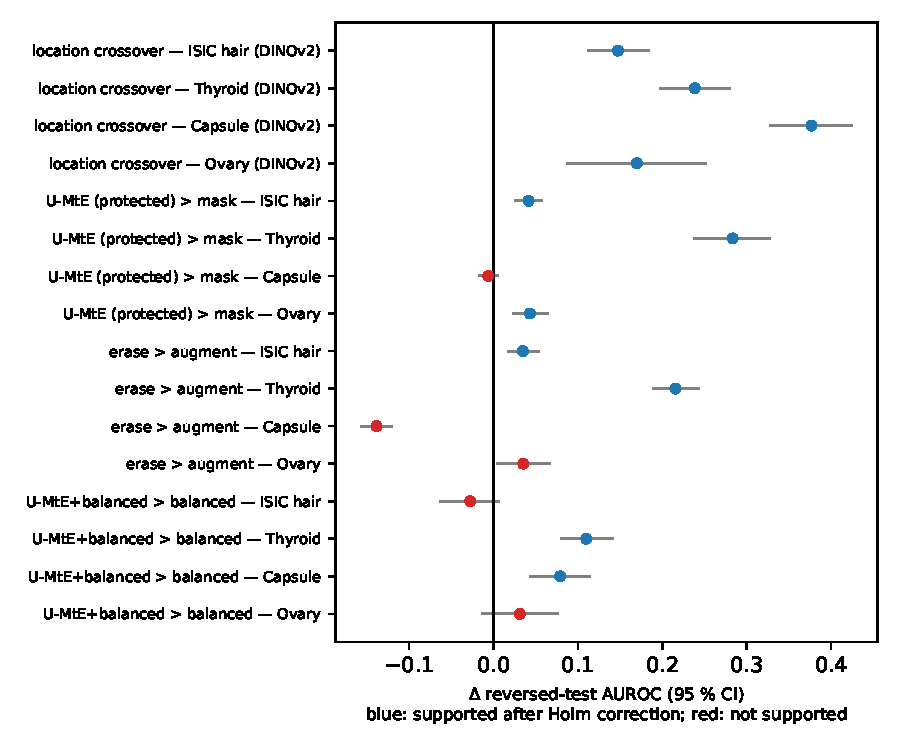
\includegraphics[width=\linewidth]{figures/forest.pdf}
\caption{The 16 pre-registered primary tests with Holm correction (blue: supported; red: not supported). Generated by
\texttt{scripts/analysis/primary\_claims.py} and \texttt{scripts/make\_figures.py}.}\label{fig:forest}\end{figure}
\fi

\paragraph{U-MtE repairs what masking leaves behind}
Without any artifact example, artifact mask or artifact label---it uses only the ROI mask that masking already
requires---U-MtE improves reversed AUROC over masking in the in-ROI regime of
every modality: thyroid calipers $+0.224$ [$+0.195, +0.253$] (DINOv2) and $+0.246$ [$+0.224, +0.269$] (MedSigLIP);
dermoscopic hair $+0.040$ [$+0.024, +0.056$]; synthetic capsule debris $+0.121$ [$+0.078, +0.170$]; synthetic
calipers $+0.278$ [$+0.214, +0.344$]; synthetic chest tubes $+0.134$ [$+0.113, +0.156$] (DINOv2 / RAD-DINO).
With MedSigLIP the unbalanced method \emph{loses} to masking in both controlled sweeps (debris $-0.190$
[$-0.265, -0.120$], calipers $-0.076$ [$-0.120, -0.034$]) although it wins on real thyroid calipers ($+0.246$);
the balanced variant beats masking at full overlap in all four controlled sweeps ($+0.211$ to $+0.470$) and has no
significant location interaction in three of them (with MedSigLIP on capsule it gains \emph{more} at full overlap:
interaction $-0.165$ [$-0.300, -0.025$]). Disease protection turns the MedSigLIP debris failure into a gain ($+0.114$
[$+0.022, +0.238$] over masking at full overlap) and the caliper one into a non-significant difference ($-0.041$
[$-0.095, +0.002$]).

\paragraph{Sensitivity to the erasure rank} In a pre-registered ablation (Trap~A, DINOv2), the thyroid gain over masking
is $+0.18$ to $+0.22$ for every setting that erases at least 16 directions (held-out energy 0.5--0.99, or fixed
$k\in\{16,64\}$), but only $+0.06$ to $+0.07$ with one to four directions: the shift caused by overlays is
multi-dimensional. The pre-specified 90\% rule reached the rank cap ($k=64$) in all three cohorts. The protected
variant never harms capsule by more than 0.010 and helps ovary at every rank ($+0.007$ to $+0.043$), whereas
unprotected erasure harms capsule more the more directions it removes, as the overlap term $\rho$ of
the linear-Gaussian account (main paper) predicts.

\paragraph{Erasure, not augmentation}
Using the same generic overlays as training augmentation (overlaid copies of a random half of the training images,
in the masked view) gains at most $+0.03$ over masking; erasing their subspace instead gains $+0.215$
[$+0.189, +0.244$] (thyroid, DINOv2), $+0.225$ [$+0.202, +0.247$] (thyroid, MedSigLIP) and $+0.035$
[$+0.017, +0.055$] (hair) more than augmentation. Under the stricter near-duplicate grouping
(main paper, stricter leakage grouping) the thyroid advantage is unchanged ($+0.192$) but the small ovary advantage
($+0.035$) loses significance, so we regard erase $>$ augment as established for thyroid and hair only.

\paragraph{When the artifact resembles the disease}
On real capsule debris U-MtE is worse than masking ($-0.126$ [$-0.146, -0.107$]): erosions carry yellow-white fibrin
that resembles debris, and a subspace estimated from real-debris templates is worse still ($-0.392$
[$-0.425, -0.360$]). Disease protection removes the failure ($-0.006$ [$-0.018, +0.006$] generic; template variant
$+0.003$ [$-0.014, +0.021$]) at no cost where erasure already works (protected minus unprotected: thyroid $+0.059$
[$+0.019, +0.096$], hair $+0.001$ [$-0.016, +0.017$]).

\paragraph{With image-level artifact labels}
Adding group balancing, U-MtE$_{\text{bal}}$ is the most robust model in thyroid ultrasound by the minimum of
correlated and reversed AUROC (0.788 DINOv2, 0.792 MedSigLIP; DFR 0.659 and 0.719); in real capsule endoscopy
masking plus last-layer retraining is higher (0.885 versus 0.857); on dermoscopic hair DFR alone is best (0.741)
because most of the hair shortcut is not in the hair pixels (removing every hair patch with the oracle mask gains
only $+0.015$). In both controlled sweeps the benefit of U-MtE$_{\text{bal}}$ no longer depends on location
(interaction $+0.021$ [$-0.019, +0.061$] capsule; $-0.053$ [$-0.108, +0.003$] thyroid), whereas that of masking
does ($+0.228$, $+0.433$).
The capsule findings replicate with MedSigLIP (crossover $+0.335$ [$+0.286, +0.383$]; masking plus DFR 0.901).
All thyroid and capsule findings replicate with a CNN (ConvNeXt-Base): crossovers $+0.275$ and $+0.320$; U-MtE $-$ mask $+0.135$ [$+0.102, +0.168$] and erase $-$ augment $+0.128$ [$+0.093, +0.161$] on thyroid.

\paragraph{Label-free and erasure baselines}
Among methods that need no artifact labels, U-MtE beats JTT \citep{liu2021jtt} by $+0.206$ [$+0.171, +0.241$]
(thyroid), $+0.125$ [$+0.063, +0.189$] (ovary) and $+0.094$ [$+0.077, +0.111$] (chest drains, RAD-DINO; not with
DINOv2, $-0.005$ [$-0.021, +0.011$]); JTT on the unmasked
view is best on hair. Task-preserving concept removal (SPLINCE; \citealp{splice2025}), fitted with artifact labels in the whitened,
minimal-distortion form of the original method, removes the artifact covariance at a large cost in disease signal
(clean AUROC 0.56--0.78 versus 0.69--0.87 for masking) and still flips the shortcut on capsule endoscopy (reversed
0.868, correlated 0.683): when artifact and label are strongly associated in training, removing one removes much of
the other. By min(reversed, correlated) U-MtE$_{\text{bal}}$ exceeds SPLINCE on thyroid, capsule and hair (0.788 vs
0.596; 0.857 vs 0.683; 0.704 vs 0.564); on chest drains SPLINCE is higher (0.609, archived run, vs 0.461) but below
DFR (0.666).

\paragraph{Text-prompted erasure}
With vision--language backbones an artifact direction can be obtained from text alone (``a thyroid ultrasound image
with measurement calipers'' minus ``a thyroid ultrasound image''; biased-prompt construction, \citealp{chuang2023debiasing}).
Erasing that subspace after masking is a near no-op in every cohort ($+0.001$ to $+0.008$ over masking; MedSigLIP
thyroid, ovary, capsule and DermLIP hair; archived runs, point estimates), whereas U-MtE with the same MedSigLIP features gains $+0.246$
[$+0.224, +0.269$] (thyroid) and $+0.210$ [$+0.167, +0.253$] (ovary). The direction along which a described artifact
moves the \emph{text} embedding is not the direction along which the real artifact moves the \emph{image} embedding;
synthetic insertions measure the latter directly.

\paragraph{A single procedure: validation-driven selection}
Selecting, per fold, the candidate with the best group-aware validation score (image-level artifact labels needed on
validation images only) beats masking in all five cohorts ($+0.17$ to $+0.40$), is within 0.02 of the best
candidate in each, and beats DFR in three (thyroid $+0.057$, capsule $+0.047$, ovary $+0.010$; archived runs, point
estimates); it chooses
U-MtE$_{\text{bal}}$ where the artifact is an overlay and plain balancing on hair and drains, where DFR remains
better. A split-validation variant that admits DFR as a candidate is reported in the supplement.

\paragraph{Modern inpainting}
Inpainting the detected caliper pixels with LaMa \citep{suvorov2022lama} and then masking is a strong baseline when
artifact masks are available (over masking: thyroid $+0.224$ [$+0.206, +0.242$], ovary $+0.128$ [$+0.084, +0.169$]).
U-MtE$_{\text{protect}}$, which needs no artifact mask, exceeds it on thyroid ($+0.060$ [$+0.013, +0.105$]) and is
below it on ovary ($-0.085$ [$-0.120, -0.050$]) and on dermoscopic hair, where published hair masks are available
($-0.086$; archived run, point estimate); with image-level artifact labels, U-MtE$_{\text{bal}}$ exceeds it in all
three ($+0.165$ [$+0.146, +0.185$], $+0.061$ [$+0.026, +0.095$], $+0.123$, archived). The thyroid comparison changed when the
run was regenerated with per-image predictions (first run: $-0.009$): the protected arm reproduced about 0.06 higher,
with unchanged code for that arm, and now agrees with the protected arm of the main regenerated run
(\texttt{results/bootstrap\_correction/archived\_old\_vs\_new.md}).

\subsection*{S8.3 End-to-end fine-tuning and erase-while-fine-tuning}
Fine-tuning ResNet-50 end-to-end (five folds) reproduces the frozen-backbone findings. Capsule: masking harms
in-ROI ($-0.279$ [$-0.377, -0.185$]) and helps out-of-ROI ($+0.301$), crossover $+0.606$ [$+0.495, +0.716$].
Thyroid: the crossover points the same way ($+0.063$ [$-0.022, +0.144$], five folds), and an end-to-end analogue of
U-MtE---an invariance penalty between masked images with and without a generic overlay---improves on masking by
$+0.139$ [$+0.096, +0.184$] without shortcut flipping (reversed 0.679, correlated 0.703), matching the best
label-using arm. It fails on capsule ($-0.021$), where the artifact resembles the pathology. Ovary (1,202 images)
is underpowered: U-MtE end-to-end has the best reversed, correlated and clean AUROC, with CIs overlapping masking.
A fine-tuned ViT-S reproduces the crossover on thyroid ($+0.122$ [$+0.039, +0.211$]), but the end-to-end U-MtE
analogue does not improve on masking with this architecture ($-0.000$ [$-0.026, +0.026$]). Applying U-MtE post hoc to
the penultimate features of the masked, fine-tuned ResNet-50 does not help either (pre-registered; $-0.000$
[$-0.001, +0.001$] over the same features without erasure): after task training the shortcut is encoded along
task-specific directions that generic overlays do not move. For fully fine-tuned networks the subspace must be
estimated and removed \emph{during} training. \emph{Erase-while-fine-tuning} (pre-registered; no artifact annotation)
projects a running estimate of the overlay-shift subspace of the network's own penultimate features out before the
head at every step and at test time, and adds feature invariance and prediction consistency between masked images with
and without a generic overlay. On thyroid it improves on masking by $+0.195$ [$+0.153, +0.237$] with ResNet-50 and
$+0.119$ [$+0.036, +0.198$] with ViT-S (reversed AUROC 0.693 and 0.608 vs 0.536 and 0.465), whereas each component
alone works for only one architecture (projection + invariance: ResNet-50 $+0.186$ [$+0.144, +0.230$], ViT-S $+0.032$
[$-0.093, +0.144$]; prediction consistency: ResNet-50 $+0.042$ [$+0.011, +0.074$], ViT-S $+0.061$ [$+0.036, +0.084$]; with the corrected
bootstrap consistency alone is now significant for both, but smaller than the combination).
With ResNet-50 the correlated AUROC falls slightly below the reversed one (0.661 vs 0.693), a mild over-correction.
On ovary (ResNet-50) it is positive but not significant ($+0.045$ [$-0.036, +0.130$]; every fine-tuning contrast on this
1,202-image cohort is underpowered), and on capsule, where debris resembles erosion fibrin, it fails ($-0.026$
[$-0.056, +0.006$]), as does every annotation-free method.

